%%%%%%%%%%%%%%%%%%%%%%%%%%%%%%%%%%%%%%%%%
% Short Sectioned Assignment LaTeX Template Version 1.0 (5/5/12)
% This template has been downloaded from: http://www.LaTeXTemplates.com
% Original author:  Frits Wenneker (http://www.howtotex.com)
% License: CC BY-NC-SA 3.0 (http://creativecommons.org/licenses/by-nc-sa/3.0/)
%%%%%%%%%%%%%%%%%%%%%%%%%%%%%%%%%%%%%%%%%

%----------------------------------------------------------------------------------------
%	PACKAGES AND OTHER DOCUMENT CONFIGURATIONS
%----------------------------------------------------------------------------------------

\documentclass[paper=a4, fontsize=11pt]{scrartcl} % A4 paper and 11pt font size

% ---- Entrada y salida de texto -----

\usepackage[T1]{fontenc} % Use 8-bit encoding that has 256 glyphs
\usepackage[utf8]{inputenc}
\usepackage{fourier} % Use the Adobe Utopia font for the document - comment this line to return to the LaTeX default

% ---- Idioma --------

\usepackage[spanish, es-tabla]{babel} % Selecciona el español para palabras introducidas automáticamente, p.ej. "septiembre" en la fecha y especifica que se use la palabra Tabla en vez de Cuadro

% ---- Otros paquetes ----

\usepackage{url} % ,href} %para incluir URLs e hipervínculos dentro del texto (aunque hay que instalar href)
\usepackage{amsmath,amsfonts,amsthm} % Math packages
%\usepackage{graphics,graphicx, floatrow} %para incluir imágenes y notas en las imágenes
\usepackage{graphics,graphicx, float} %para incluir imágenes y colocarlas
\usepackage{epstopdf}
\usepackage[gen]{eurosym} %para incluir el símbolo del euro
\usepackage{cite} %para incluir citas del archivo <nombre>.bib
%\graphicspath{/images}

% Para hacer tablas comlejas
%\usepackage{multirow}
%\usepackage{threeparttable}

%\usepackage{sectsty} % Allows customizing section commands
%\allsectionsfont{\centering \normalfont\scshape} % Make all sections centered, the default font and small caps

\usepackage{fancyhdr} % Custom headers and footers
\pagestyle{fancyplain} % Makes all pages in the document conform to the custom headers and footers
\fancyhead{} % No page header - if you want one, create it in the same way as the footers below
\fancyfoot[L]{} % Empty left footer
\fancyfoot[C]{} % Empty center footer
\fancyfoot[R]{\thepage} % Page numbering for right footer
\renewcommand{\headrulewidth}{0pt} % Remove header underlines
\renewcommand{\footrulewidth}{0pt} % Remove footer underlines
\setlength{\headheight}{13.6pt} % Customize the height of the header

\numberwithin{equation}{section} % Number equations within sections (i.e. 1.1, 1.2, 2.1, 2.2 instead of 1, 2, 3, 4)
\numberwithin{figure}{section} % Number figures within sections (i.e. 1.1, 1.2, 2.1, 2.2 instead of 1, 2, 3, 4)
\numberwithin{table}{section} % Number tables within sections (i.e. 1.1, 1.2, 2.1, 2.2 instead of 1, 2, 3, 4)

\setlength\parindent{0pt} % Removes all indentation from paragraphs - comment this line for an assignment with lots of text

\newcommand{\horrule}[1]{\rule{\linewidth}{#1}} % Create horizontal rule command with 1 argument of height


%----------------------------------------------------------------------------------------
%	TÍTULO Y DATOS DEL ALUMNO
%----------------------------------------------------------------------------------------

\title{
\normalfont \normalsize
\textsc{\textbf{Ingeniería de Servidores (2016-2017)} \\ Grado en Ingeniería Informática \\ Universidad de Granada} \\ [25pt]
\horrule{0.5pt} \\[0.4cm]
\huge Memoria Práctica 5 \\
\horrule{2pt} \\[0.5cm]
}

\author{Adrián Morente Gabaldón}
\date{\normalsize\today}

%----------------------------------------------------------------------------------------
% DOCUMENTO
%----------------------------------------------------------------------------------------

\begin{document}

\maketitle % Muestra el Título

\newpage %inserta un salto de página

\tableofcontents % para generar el índice de contenidos

\newpage

\listoffigures

\listoftables

\newpage


\section{[SYSCTL] Al modificar los valores del kernel de este modo, no logramos que persistan después de reiniciar la máquina. ¿Qué archivo hay que editar para que los cambios sean permanentes?}
Como ya se explicó en clase de prácticas, \emph{Sysctl} modifica los parámetros del kernel en tiempo de ejecución, por lo que al reiniciar la máquina se pierden los valores modificados. Si ejecutamos Sysctl a través de línea de comandos sin opciones, se nos despliega una pequeña lista con sus opciones más destacadas, que son las siguientes:
\begin{figure}[H]
	\centering
	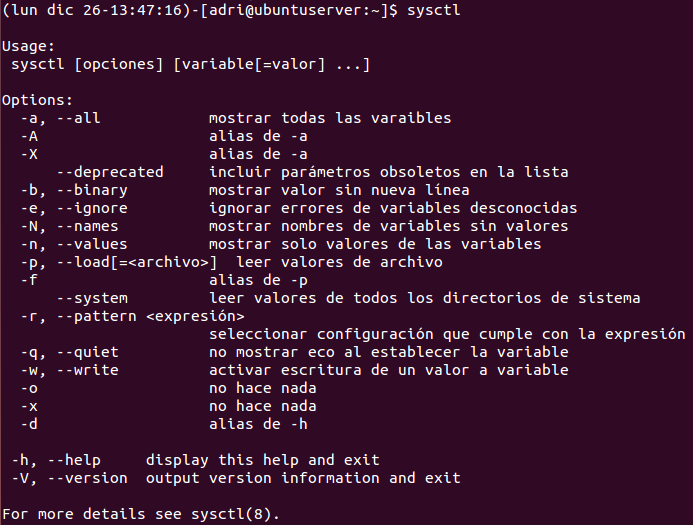
\includegraphics[scale=0.6]{sysctl-h}
	\caption{Opciones más destacadas de sysctl. - Adrián Morente Gabaldón [26/12/2016]}
	\label{figura1}
\end{figure}
Como vemos en la captura de pantalla anterior, el propio sysctl nos redirige a su manual si queremos explorar más opciones u obtener más información. Al principio de este manual, encontramos que todos los parámetros configurables descienden del directorio \emph{/proc/sys}, ordenados en subcarpetas según pertenencia (sistema de archivos, kernel, memoria virtual, etc), y cada uno de ellos se encuentra en formato de archivo en texto plano, conteniendo tan solo el valor del parámetro en cuestión. Veamos un ejemplo de los parámetros pertenecientes al módulo de memoria virtual:
\begin{figure}[H]
	\centering
	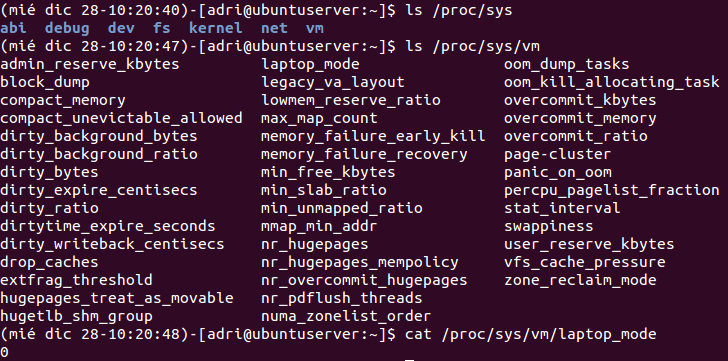
\includegraphics[scale=0.7]{proc-sys}
	\caption{Contenido del directorio /proc/sys, sus subdirectorios y ejemplo de uno de sus parámetros. - Adrián Morente Gabaldón [28/12/2016]}
	\label{figura3}
\end{figure}
Para que los cambios persistan tras reiniciar la máquina, debemos aplicar la modificación a cada uno de los ficheros de parámetros. Sin embargo, por temas de seguridad, es mejor utilizar esta herramienta con algunas de sus múltiples opciones en lugar de acceder y modificar directamente dichos ficheros (ya que podemos ``tocar donde no debemos''), cosa que podría derivar en algún fallo no deseado del sistema.\\
Como vimos en clase, y como bien comenta el manual de \emph{sysctl}, la configuración perteneciente y valorable por esta herramienta se encuentra principalmente en el archivo /etc/sysctl.config, y colgando del directorio /etc/sysctl.d. Veamos una parte del contenido de dicho primer archivo:
\begin{figure}[H]
	\centering
	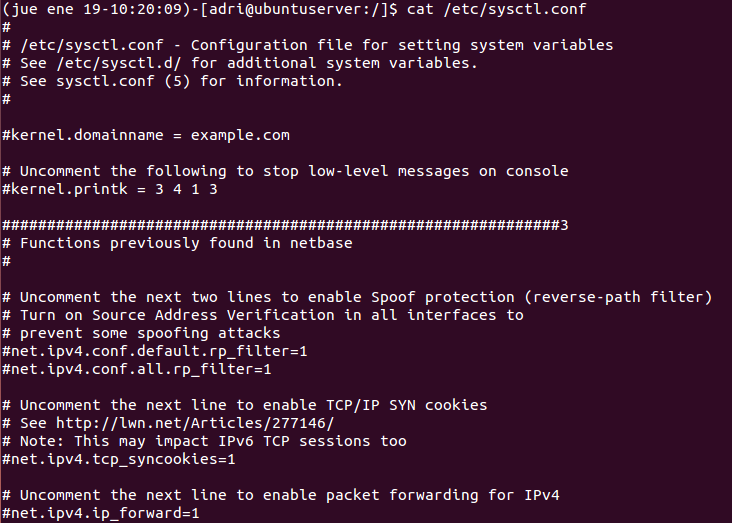
\includegraphics[scale=0.36]{sysctl-conf}
	\caption{Parte del contenido del archivo de configuración /etc/sysctl.config. - Adrián Morente Gabaldón [19/01/2017]}
	\label{figura5}
\end{figure}
Como podemos apreciar, no encontramos mucha información sobre qué es cada cosa, solo encontramos nombres de variables con sus correspondientes valores; todos ellos ordenados de forma clara y precisa según su ámbito. Por ejemplo, veamos uno de estos ámbitos que, personalmente, me ha llamado la atención, y es el relacionado con la \textbf{seguridad} del sistema:
\begin{figure}[H]
	\centering
	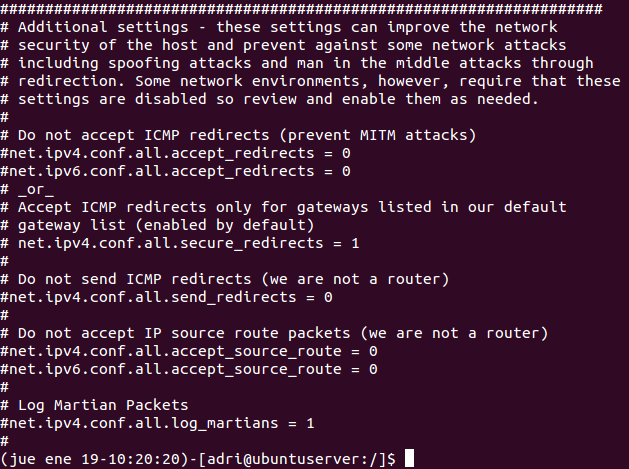
\includegraphics[scale=0.45]{sysctl-security}
	\caption{Contenido del archivo de configuración /etc/sysctl.config relacionado con la seguridad del sistema. - Adrián Morente Gabaldón [19/01/2017]}
	\label{figura6}
\end{figure}
En este apartado, encontramos parámetros configurables que nos permitirían en cierto modo evitar algunos ataques a nuestro sistema, como pueden ser el bloqueo de redirecciones mediante el protocolo ICMP (que incluye herramientas como ping o traceroute, como hemos visto en la asignatura de \emph{Fundamentos de Redes}). Como bien explica la pequeña introducción en este apartado, estas son medidas contra el \emph{spoofing} (que en español se traduce por \emph{burla} o \emph{engaño}, y en informática entendemos por ``falsificación de identidad'') y contra ataques \emph{Man In The Middle}, término que ya conocemos.\\
Para terminar, cabe destacar que todos estos últimos parámetros están comentados, de forma que el sistema toma valores por defecto en caso de que no sean modificados aquí. Las instrucciones del archivo nos instan a no modificar parámetros si no sabemos lo que estamos haciendo. Además, ya sabemos que en caso de tener que modificarlos, debemos hacer copia de seguridad previa a su modificación.


\section{¿Con qué opción se muestran todos los parámetros modificables en tiempo de ejecución? Elija dos parámetros y explique, en dos líneas, qué función tienen.}
Si leemos el manual de sysctl en la terminal, vemos rápidamente que la opción para consultar todas las variables modificables en ejecución es \emph{-a} (o \emph{--all}, si lo preferimos):
\begin{figure}[H]
	\centering
	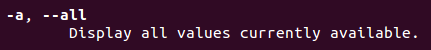
\includegraphics[scale=0.7]{sysctl-a}
	\caption{Opción de Sysctl para consultar los parámetros modificables en ejecución. - Adrián Morente Gabaldón [26/12/2016]}
	\label{figura2}
\end{figure}
Si ejecutamos \textbf{sysctl -a} obtenemos una extensa lista con todas las variables configurables. Exactamente, tantas como ficheros había en los subdirectorios de \emph{/proc/sys} vistos en el ejercicio anterior, lógicamente.
	\subsection{Parámetro ``vm\_laptop\_mode''.}
	Como vemos en la documentación oficial de \emph{kernel.org} \cite{kernel-laptop}, el \emph{laptop\_mode} (o ``modo portátil'') consiste en una subherramienta del kernel que permite a sistemas Unix ahorrar batería (iniciando automáticamente el sistema en este modo), a partir de intentar minimizar 	el número de rotaciones que realiza el disco duro. Está desactivado por defecto (a 0).
	\subsection{Parámetro ``kernel\_sched\_nr\_migrate''.}
	Según la documentación oficial de SUSE (conocidísima distribución de GNU/Linux) \cite{kernel-sched}, este parámetro se aplica directamente al número de tareas que pueden intercambiarse entre procesos durante una interrupción de software. El valor por defecto es 32. Aumentar este número aumenta el rendimiento en hebras con tareas largas, pero incrementa la latencia para tareas en tiempo real.


\section{[Windows Server] a) Realice una copia de seguridad del registro y restáurela, ilustre el proceso con capturas. b) Abra una ventana mostrando el editor del registro.}
	\subsection{a) Realice una copia de seguridad del registro y restáurela, ilustre el proceso con capturas.}
	Para empezar, seguiremos las instrucciones dictadas por el guión de prácticas, y veremos que es extremadamente fácil (como prácticamente todo en Windows) 	comenzando por ejecutar \emph{regedit}	desde la línea de comandos de Windows Server. A continuación, nos encontraremos con esta ventana:
	\begin{figure}[H]
		\centering
		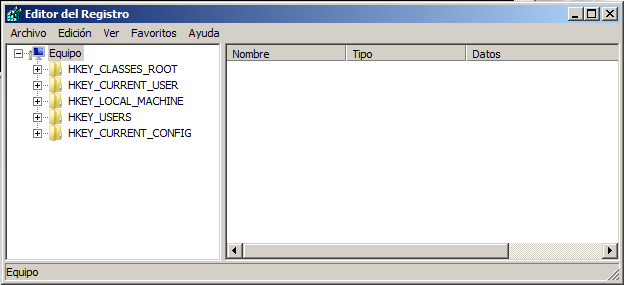
\includegraphics[scale=0.7]{regedit}
		\caption{Ventana principal del Editor del Registro en Windows Server. - Adrián Morente Gabaldón [26/12/2016]}
		\label{figura4}
	\end{figure}
	Acto seguido, en la pestaña ``Archivo'' veremos disponibles las dos opciones que requiere esta cuestión (Importar -> Exportar). Empezaremos con la exportación del registro, seleccionando dicha opción:
	\begin{figure}[H]
		\centering
		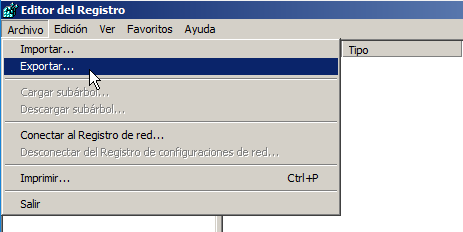
\includegraphics[scale=0.8]{regedit-exportar}
		\caption{Exportación del registro en Windows Server. - Adrián Morente Gabaldón [19/01/2017]}
		\label{figura7}
	\end{figure}
	Fácilmente, elegimos el nombre deseado del archivo y su ubicación:
	\begin{figure}[H]
		\centering
		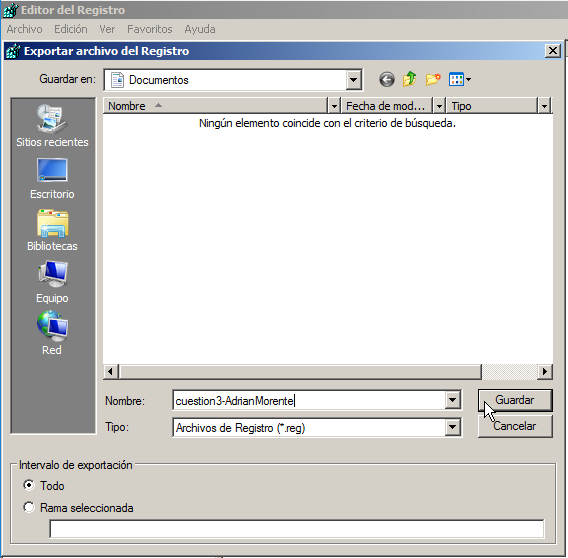
\includegraphics[scale=0.8]{regedit-exportar2}
		\caption{Exportación del registro en Windows Server. - Adrián Morente Gabaldón [19/01/2017]}
		\label{figura8}
	\end{figure}
	El segundo paso, a la hora de importar dicha copia previamente realizada, seguiremos un proceso muy similar pero a la inversa, seleccionando la opción de 	``Importar'' y escogiendo el archivo a importar del directorio correspondiente:
	\begin{figure}[H]
		\centering
		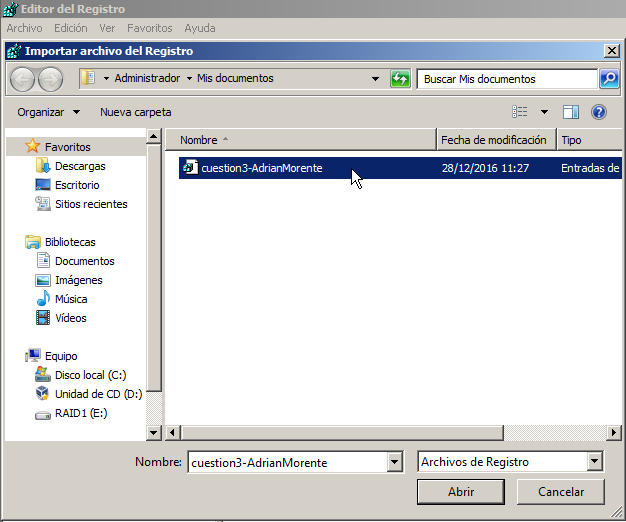
\includegraphics[scale=0.7]{regedit-importar}
		\caption{Importación del registro en Windows Server. - Adrián Morente Gabaldón [19/01/2017]}
		\label{figura9}
	\end{figure}
	A continuación, para terminar, nos aparecerá una sencilla barra de carga mostrando el rápido proceso de importación de dicha copia.
	\begin{figure}[H]
		\centering
		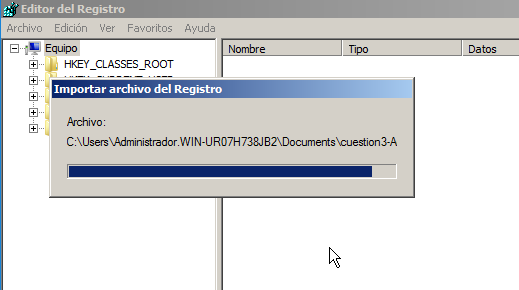
\includegraphics[scale=0.7]{regedit-importar2}
		\caption{Importación del registro en Windows Server. - Adrián Morente Gabaldón [19/01/2017]}
		\label{figura10}
	\end{figure}

	\subsection{b) Abra una ventana mostrando el editor del registro.}
	Como bien sabemos, además de lo que explica el guión de la práctica, en el registro de Windows podemos encontrar configuraciones de todo tipo, ya sean sobre el hardware o el software. Una buena práctica como administradores de sistemas, sería hacer una copia de seguridad previa a cualquier modificación, como bien hemos hecho en el primer apartado de esta cuestión. Una vez hecho esto, somos ``libres'' de realizar cualquier cambio, siempre a sabiendas de qué estamos tocando. Una ventana de ejemplo del registro sería ésta:
	\begin{figure}[H]
		\centering
		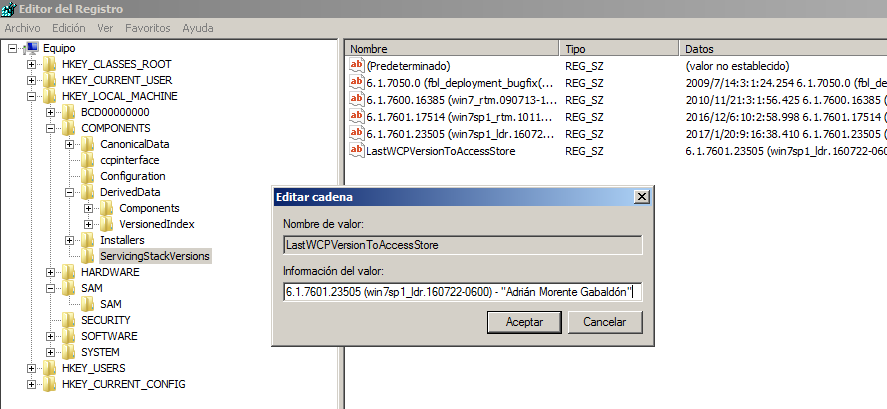
\includegraphics[scale=0.45]{regedit-example}
		\caption{Ejemplo del editor del registro en Windows Server. - Adrián Morente Gabaldón [19/01/2017]}
		\label{figura11}
	\end{figure}
	Como podemos apreciar en el árbol de la izquierda, las configuraciones del equipo se subdividen en varias colmenas:
	\begin{itemize}
		\item Configuraciones del usuario \emph{root} o ``Administrador''.
		\item Parámetros pertenecientes al usuario actual.
		\item Parámetros pertenecientes al hardware y software de la máquina.
		\item Variables correspondientes al resto de usuarios del sistema (en este caso, solo existe uno, que es el Administrador).
		\item Configuración actual del sistema (fuentes, impresoras predeterminadas, etc.).
	\end{itemize}
	Sin embargo, en cuanto empecemos a buscar un poco de documentación oficial de Windows sobre qué hace cada registro, nos damos de bruces con la realidad de Microsoft, y es que existe mucho ocultismo por su parte en cuanto a la configuración a bajo nivel de sus sistemas. De hecho, cuando intentamos consultar la Ayuda del Registro que ellos mismos proporcionan, encontramos instrucciones muy básicas sobre cómo actuar, pero ninguna explicación del significado de cada parámetro:
	\begin{figure}[H]
		\centering
		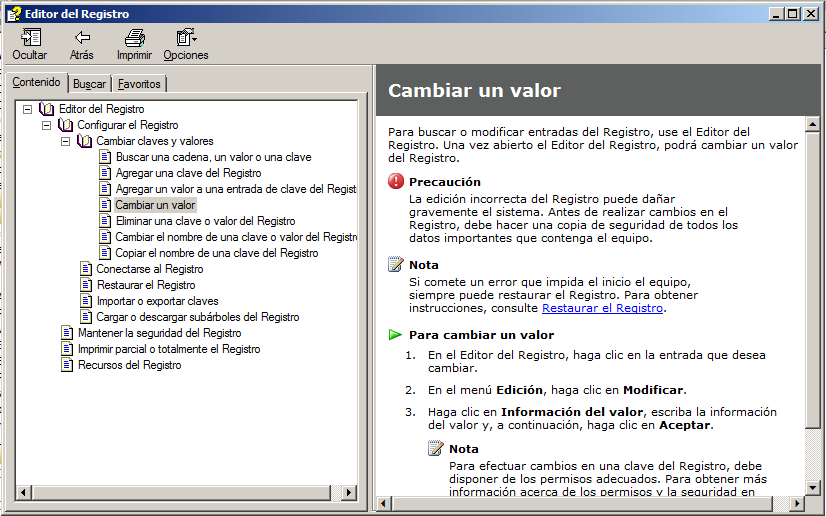
\includegraphics[scale=0.5]{regedit-help}
		\caption{Ayuda del registro en Windows Server. - Adrián Morente Gabaldón [19/01/2017]}
		\label{figura12}
	\end{figure}



\section{Enumere qué elementos se pueden configurar en Apache y en IIS para que Moodle funcione mejor.}
Si seguimos el enlace a la web de Moodle proporcionado por el guión de la práctica, veremos que en ella nos proponen usar la nueva documentación, para la versión actual (3.2), en lugar de la versión antigua (2.3) que se propone en dicho guión. Sin embargo, tras comparar las secciones que nos interesan (rendimiento en Apache y en IIS) vemos que el contenido es idéntico, por lo que podremos usar cualquiera de ellas indistintamente. \\
En dicha documentación oficial nos instan a realizar las siguientes acciones, en aras de que el servicio desempeñe un mejor rendimiento. Todas ellas son fácilmente realizables, ya que solo consisten en alterar ciertos valores del registro del sistema en Windows Server; y añadir o modificar algunas líneas de código a ciertos archivos de configuración en Linux.

	\subsection{Mejora de rendimiento de Moodle en IIS}
	Toda la configuración para mejorar el rendimiento en Windows, como ya hemos dicho, consiste en modificar algunos valores de registros. No debemos olvidar 	que antes de hacer esto, estamos ``obligados'' a realizar una copia de seguridad del registro, igual que en el ejercicio anterior, de forma que podamos 			\emph{volver atrás} si erramos en algo. Toda la configuración deberá ser aplicada al registro \emph{HKLM\textbackslash SYSTEM\textbackslash 					CurrentControlSet\textbackslash Services\textbackslash Inetinfo\textbackslash Parameters\textbackslash}, según nos indica Moodle \cite{moodle-iis}:
	\begin{itemize}
		\item Cambiar el parámetro \emph{ListenBackLog} de 2 a 5. Esto configura el tiempo de espera en conexión tras responder a una petición del cliente. Se aprovecha la misma conexión para enviar más datos y ahorrar tiempo de cierre+reapertura de conexión.
		\item Cambiar la memoria caché que usará IIS por defecto al 50\% de la memoria total del sistema en el parámetro \emph{MemCacheSize}.
		\item Cambiar el tamaño máximo de memoria de caché para un archivo en el parámetro \emph{MaxCachedFileSize} a 256KiB.
		\item Crear un nuevo parámetro (\emph{DWORD}) llamado \emph{ObjectCacheTTL}, que contendrá el tiempo máximo que un archivo estará cargado en la memoria caché del servidor. Estableceremos el valor a 30.000 milisegundos (30 segundos).
	\end{itemize}

	\subsection{Mejora de rendimiento de Moodle en Apache}
	Al contrario que en IIS, la configuración para Apache es algo más compleja, y si bien la documentación de Moodle al respecto es extensa, la complejidad que aporta no es pequeña, dada la escasa especificidad con la que se explican los cambios a aplicar. Para solucionar esto, habré instalado Moodle sobre Apache en Ubuntu Server, de forma que además de tener todos los archivos de configuración accesibles, podremos hacer un estudio de rendimiento posterior a los cambios para la cuestión 6 de este guión.\\
	Para empezar, si indagamos en los pasos de instalación y configuración de Moodle sobre Apache encontraremos lo siguiente:
	\begin{figure}[H]
		\centering
		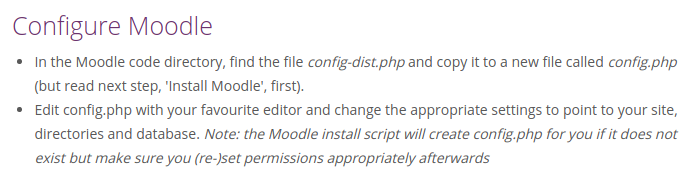
\includegraphics[scale=0.5]{pasos-moodle}
		\caption{Procedimiento para configurar los parámetros de Moodle sobre Apache en Linux. - Adrián Morente Gabaldón [19/01/2017]}
		\label{figura13}
	\end{figure}
	Estas instrucciones nos instan a copiar el archivo \emph{config-dist.php} con el nombre \emph{config.php}, el cual configuraremos con el editor de texto que más nos guste, modificando en él los aspectos esenciales como el sitio web, aspectos de la base de datos, etc. Aquí será donde apliquemos los cambios para mejorar su rendimiento, de los que destacaremos los siguientes, según la primera guía que veíamos de Moodle \cite{moodle-apache}:
	\begin{itemize}
		\item Ajustaremos el número máximo de usuarios (parámetro \emph{MaxClients}) exactamente al 80\% de la memoria disponible del sistema. Si asignamos más memoria de la disponible realmente, Moodle comenzará a consumir memoria de intercambio del disco.
		\item Para reducir la memoria consumida, reduciremos el número de módulos cargados por defecto en el archivo \emph{httpd.conf}, desactivando los que no necesitemos utilizar (u ofrecer).
		\item Usaremos siempre la última versión de Apache (como solemos hacer y es recomendado con cualquier software), Apache2, ya que contiene mejoras como por ejemplo, el aprovechamiento de la memoria del sistema.
		\item Si no utilizamos control de accesos con el fichero \emph{.htaccess}, cambiaremos el valor del parámetro \emph{AllowOverride} a ``None'', de forma que evitemos la consulta constante a este archivo.
		\item Si no estamos realizando ningún tipo de desarrollo en el servidor, pondremos el estado \emph{ExtendedStatus} en \emph{Off}, desactivando \emph{mod-info} y \emph{mod-status}.
		\item Reduciremos el valor de \emph{TimeOut} a 30-60 segundos, de forma que se interrumpan las conexiones que excedan de este tiempo, liberando la carga del servidor.
		\item Para reducir la carga de entrada/salida ajustaremos la directiva \emph{Options} con el contenido ``Options -Indexes FollowSymLinks'', de forma que el escaneado de directorios siga enlaces simbólicos en su búsqueda de ficheros.
		\item Para reducir el tiempo de respuestas HTTP, ya sabemos que podemos comprimir el tamaño de dichas respuestas. Para ello, instalamos \emph{mod- deflate} \cite{mod-deflate} y lo activamos. A continuación, añadimos al fichero de configuración el fragmento de código aportado por la documentación de Moodle.org:
		\begin{verbatim}
		<ifModule mod_deflate.c>
  		    AddOutputFilterByType DEFLATE text/html text/plain text/xml
		</ifmodule>
		\end{verbatim}
	\end{itemize}


\section{Ajuste la compresión en el servidor y analice su comportamiento usando varios valores para el tamaño de archivo a partir del cual comprimir. Para comprobar que está comprimiendo puede usar el navegador o comandos como curl (see url) o lynx. Muestre capturas de pantalla de todo el proceso.}


\section{a) Usted parte de un SO con ciertos parámetros definidos en la instalación (Práctica 1), ya sabe instalar servicios (Práctica 2) y cómo monitorizarlos (Práctica 3) cuando los somete a cargas (Práctica 4). Al igual que ha visto cómo se puede mejorar un servidor web (Práctica 5 Sección 3.1), elija un servicio (el que usted quiera) y modifique un parámetro para mejorar su comportamiento. b) Monitorice el servicio antes y después de la modificación del parámetro aplicando cargas al sistema (antes y después) mostrando los resultados de la monitorización.}



\bibliography{citas}
\bibliographystyle{plain}

\end{document}
